\chapter{Opis struktury projektu}
\label{chap:Opis struktury projektu}

\section{Wykorzystane technologie i narzędzia}
\label{sec:Struktura projektu}
Sercem aplikacji jest język \textbf{Java}. To, co użytkownik widzi na ekranie, czyli interfejs graficzny, to zasługa biblioteki \textbf{Java Swing}. Wszystkie dane - o produktach, klientach czy zamówieniach - trafiają do bazy danych \textbf{MySQL}, a „mostem”, który łączy aplikację z bazą, jest technologia \textbf{JDBC}.

Nad całym kodem i historią jego zmian czuwał system kontroli wersji \textbf{Git}, a jego centralne repozytorium znajdowało się na platformie \textbf{GitHub}. Cały proces programowania odbywał się w środowisku \textbf{IntelliJ IDEA}.

\section{Architektura i hierarchia klas}
Aplikacja została zbudowana z wykorzystaniem trójwarstwowej architektury, co zapewnia czytelny podział odpowiedzialności pomiędzy komponentami systemu. Każda warstwa ma ściśle określone zadania i komunikuje się z innymi poprzez dobrze zdefiniowane interfejsy.

\begin{enumerate}
    \item \textbf{Warstwa prezentacji (GUI)} - znajduje się w pakietach \texttt{gui} oraz \texttt{bazowe}:
    \begin{itemize}
        \item \texttt{MenuGlowne.java} - główne menu aplikacji
        \item \texttt{OknoLogowania.java} - formularz logowania
        \item \texttt{OknoRejestracji.java} - formularz rejestracji
        \item \texttt{PanelAdministratora.java} - panel administratora
        \item \texttt{PanelUzytkownika.java} - panel zwykłego użytkownika
        \item \texttt{OknoBazowe.java} - abstrakcyjna klasa bazowa dla okien
    \end{itemize}
    
    \item \textbf{Warstwa logiki biznesowej} - pakiet \texttt{serwis}:
    \begin{itemize}
        \item \texttt{Produkty.java} - zarządzanie produktami i rezerwacjami
        \item \texttt{Kary.java} - obsługa kar za przekroczenie czasu magazynowania
        \item \texttt{PrzychodyMagazynu.java} - zarządzanie przychodami
        \item \texttt{UzytkownikSerwis.java} - operacje na użytkownikach
    \end{itemize}
    
    \item \textbf{Warstwa dostępu do danych} - pakiet \texttt{BazaDanych}:
    \begin{itemize}
        \item \texttt{DatabaseConnector.java} - połączenie z bazą danych
        \item Wspierana przez klasy z pakietu \texttt{narzedzia} (\texttt{Walidacja.java})
    \end{itemize}
\end{enumerate}
\clearpage
\section{Baza danych}
\label{sec:Baza danych}
Wszystkie dane przechowywane są w relacyjnej bazie danych. Znajdują się w niej takie tabele jak: uzytkownicy, transakcje, produkty oraz kary.

\begin{figure}[H]
    \centering
    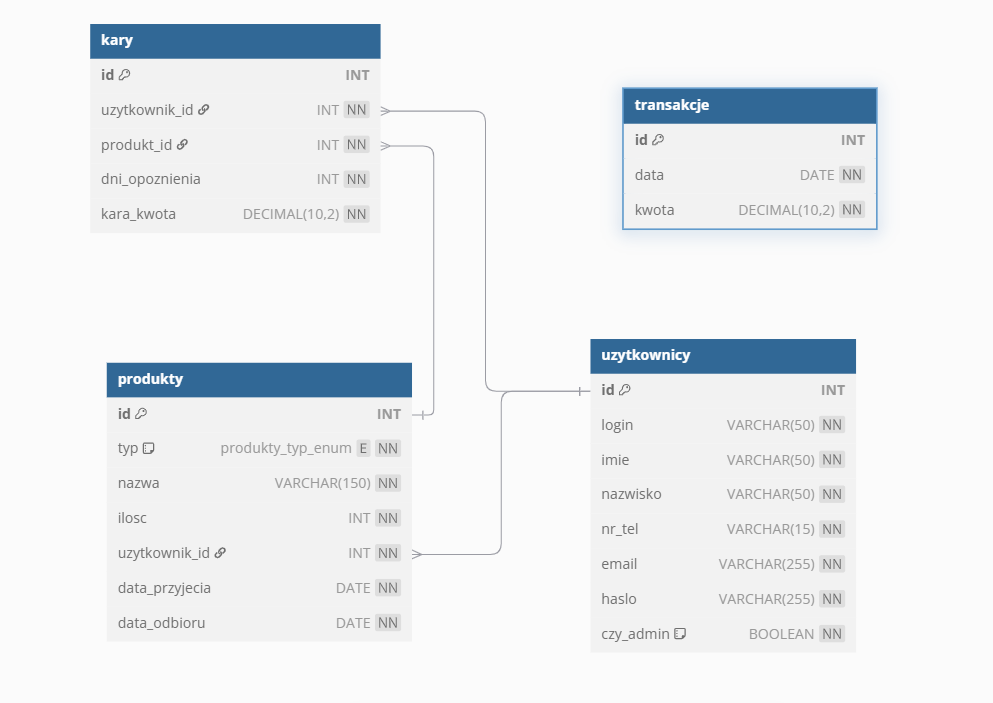
\includegraphics[width=.7\linewidth]{figures/SchematERD.png}\
    \caption{SchematERD.\label{schematERD}}
\end{figure}

\section{Kluczowe zależności oraz charakterystyka architektury}
\begin{itemize}
    \item \textbf{Dziedziczenie} - Wszystkie główne okna dziedziczą po \texttt{OknoBazowe}, co zapewnia spójny wygląd i zachowanie interfejsu użytkownika
    \item \textbf{Kompozycja} - Klasy serwisowe są używane przez panele użytkownika i administratora, a \texttt{DatabaseConnector} przez wszystkie klasy potrzebujące dostępu do bazy danych.
    \item \textbf{Modułowość} - Każda warstwa może być modyfikowana niezależnie od innych
    \item \textbf{Testowalność} - Logikę biznesową można testować w izolacji od warstwy prezentacji i danych
    \item \textbf{Spójność interfejsu} - Dzięki dziedziczeniu z \texttt{OknoBazowe} wszystkie okna mają jednolity wygląd
    \item \textbf{Bezpieczeństwo} - Walidacja danych na poziomie GUI i logiki biznesowej
\end{itemize}
\clearpage
\section{Wymagania systemowe}
Aby uruchomić projekt na własnym komputerze i móc go rozwijać, potrzebne jest kilka darmowych narzędzi. Poniższa lista wyjaśnia, co i dlaczego należy zainstalować.
\begin{itemize}
    \item \textbf{Pakiet XAMPP:} To gotowy zestaw narzędzi, który w prosty sposób instaluje serwer bazy danych. Jest on niezbędny, aby aplikacja miała gdzie przechowywać swoje dane.
    \item \textbf{Java Development Kit (JDK):} Jest to środowisko niezbędne do kompilowania i uruchamiania aplikacji napisanych w języku Java.
    \item \textbf{Środowisko IntelliJ IDEA:} To zaawansowany edytor kodu, w którym projekt był tworzony. Ułatwia on pracę z kodem, kompilację i uruchamianie programu.
\end{itemize}
Aktualne wymagania sprzętowe dla tych programów można znaleźć na ich oficjalnych stronach:
\begin{itemize}
    \item \textbf{XAMPP:} \url{https://www.apachefriends.org/download.html}
    \item \textbf{IntelliJ IDEA:} \url{https://www.jetbrains.com/help/idea/installation-guide.html#requirements}
\end{itemize}
